\documentclass[xcolor=dvipsnames,compress]{beamer}

%\usepackage{amssymb,amsmath} 
\usepackage{verbatim}

% global beamer options
\usetheme{Warsaw}
\usecolortheme[RGB={180,20,30}]{structure} 
\setbeamertemplate{items}[triangle] 
\setbeamertemplate{blocks}[rounded][shadow=true]
\setbeamertemplate{section in toc}[square]
\setbeamertemplate{subsection in toc}[square]
%\setbeamercovered{dynamic}

\usepackage{ccicons}
% diagrams
%\usepackage{pstricks}
\usepackage{graphicx}

% code highlighting
\usepackage{minted}
\usemintedstyle{tango}
% seems we need this for add a label to framed code (fancyvrb - minted issue)
\makeatletter
\minted@define@extra{label}
\makeatother

\usepackage[absolute,overlay]{textpos} 
\newenvironment{reference}[2]{% 
  \begin{textblock*}{\textwidth}(#1,#2) 
      \tiny\it\bgroup\color{blue}}{\egroup\end{textblock*}} 

\newcommand\Fontvi{\fontsize{6}{7.2}\selectfont}

\newminted{c}{gobble=4,fontsize=\tiny,frame=single,rulecolor=\structure}
\newminted{make}{gobble=4,fontsize=\tiny,frame=single,rulecolor=\structure}
%\newminted{cpp}{gobble=4,fontsize=\tiny,frame=single}
%\newminted{xml}{gobble=4,fontsize=\tiny,frame=single}
%\newminted{sql}{gobble=4,fontsize=\tiny,frame=single}


\title[linux device drivers intro]{Linux Device Drivers}
\subtitle{A crash course (from a novice)}
\author{Alexandre Moreno}
\institute[Seenergy]{SEEnergy Corp.\\
   \texttt{alexandre@seenergy.com.tw}
} 
\subject{talk}
\date{\today}
%\logo{\includegraphics[height=1.0cm]{../Company_Logo.png}}
\titlegraphic{\ccbysa}

\begin{document}

\begin{frame}[plain]
   \titlepage
\end{frame}

\section*{outline}
\begin{frame}
   \tableofcontents
\end{frame}

\section[intro]{Introduction}
\begin{frame}
\frametitle{Introducton}
    \structure{Device drivers} are the abstraction layer between software concepts and hardware circuitry:
    \begin{itemize}
    \item They provide a standard interface to perihperals, hiding the details of how devices work
    \item Almost every system operation eventually maps to a physical device
    \item The OS kernel embeds device drivers for every peripheral device present in the system
    \item Unix motto also applies here, i.e. provide mechanism, not policy
    \item In the Linux kernel 2.4.1 device driver code accounts for about 70\% of the code size
    \end{itemize}
\end{frame}

\begin{frame}
\frametitle{Classes of devices}
    Typically device drivers are classified as follows:
    \begin{itemize}
    \item \structure{Character devices}: they are accessed as a stream of bytes (like a file); a char driver is in charge of implementing such behaviour
    \item \structure{Block devices}: I/O operations transfer whole blocks (e.g. 512 bytes), and can host a filesystem. Example is /dev/sda
    \item \structure{Network interfaces}\\
    \end{itemize}
    But this taxonomy is not universal, e.g. an USB device might appear in the kernel as char device (serial port), 
    block device (USB flash drive) or network device (USB Ethernet interface)\\
\end{frame}

\begin{frame}[fragile]
\frametitle{Loadable Modules}
    \begin{itemize}
    \item Linux has the ability to extend the kernel functionality at runtime using modules
    \item Device drivers can also be added to the kernel in this fashion (benefits are a smaller kernel, on demand loading gives you a better footprint and no  kernel recompilation to add new modules)
    \item You can use the \structure{module-init-tools} package, which contains a set of programs for loading, inserting and removing kernel modules.
    \end{itemize}
    \Fontvi
    \begin{verbatim}
    Example:
        obj-$(CONFIG_FOO) += foo.o

      $(CONFIG_FOO) evaluates to either y (for built-in) or m (for module).
      If CONFIG_FOO is neither y nor m, then the file will not be compiled
      nor linked.
    \end{verbatim}
\end{frame}

\section[hello]{Hello, world}
\begin{frame}[fragile]
\frametitle{hello, world (1)}
    \begin{ccode*}{label=helloworld.c} 
    #include <linux/init.h>
    #include <linux/module.h>
    MODULE_LICENSE("Dual BSD/GPL");

    static int hello_init(void)
    {
        printk(KERN_ALERT "Hello, world\n");
        return 0;
    }

    static void hello_exit(void)
    {
        printk(KERN_ALERT "Goodbye, world\n");
    }

    module_init(hello_init);
    module_exit(hello_exit);
    \end{ccode*}
    \begin{makecode*}{label=Makefile}
    ifneq ($(KERNELRELEASE),)
        obj-m := helloworld.o
    else
        KERNELDIR ?= /lib/modules/$(shell uname -r)/build
        PWD := $(shell pwd)
    default:
        $(MAKE) -C $(KERNELDIR) M=$(PWD) modules
    endif
    \end{makecode*}
\end{frame}
\begin{frame}[fragile]
\frametitle{hello, world (2)}
    And this is a simple session showing how to bring it to life
    \Fontvi
    \begin{verbatim}
    $ ls
    helloworld.c  helloworld.ko  helloworld.mod.c  helloworld.mod.o  
    helloworld.o  Makefile  modules.order  Module.symvers

    $ sudo insmod ./helloworld.ko
    $ dmesg | tail -1
    [151235.953044] Hello, world

    $ cat /proc/modules | grep helloworld
    helloworld 680 0 - Live 0xf8252000

    $ modinfo helloworld.ko
    filename:       helloworld.ko
    license:        Dual BSD/GPL
    srcversion:     736D100661E927970863868
    depends:        
    vermagic:       2.6.32-39-generic SMP mod_unload modversions 586 

    $ sudo rmmod helloworld 
    $ dmesg | tail -1
    [151277.360643] Goodbye, world
    \end{verbatim}
\end{frame}

\section[ABI]{Kernel Space - User Space Interfaces}
\begin{frame}
    Linux provides different mechanism for communicating between user and kernel space:
    \begin{itemize}
    \item System calls (functions which are useful for \_many\_ application programs)
    \item ioctl system call
    \item Virtual file systems (\structure{procfs}, sysfs, configfs, debugfs)
    \item sysctl
    \item Netlink sockets
    \item Upcall
    \end{itemize}
\end{frame}

\begin{frame}[fragile]
    \frametitle{Access the Linux kernel using the /proc filesystem}
    \begin{ccode*}{label=prochello.c} 
    #include <linux/init.h>
    #include <linux/module.h>
    #include <linux/proc_fs.h>  /* Necessary because we use the proc fs */

    static struct proc_dir_entry *proc_ent;
    static int proc_read(char *buffer, char **start, off_t offset, int size, int *eof, void *data)
    {
      char *hello_str = "Hello, world!\n";
      int len = strlen(hello_str); /* Don't include the null byte. */
      strcpy(buffer, hello_str);
      *eof = 1;
      return len;
    }
    static int simpl_init(void)
    {
      proc_ent = create_proc_entry("simpl", 0, NULL);
      if(!proc_ent){
        remove_proc_entry("simpl", NULL/*&proc_root*/);
        return -ENOMEM;
      }
      proc_ent->read_proc = proc_read;
      return 0;
    }
    static void simpl_exit(void)
    {
      remove_proc_entry("simpl", NULL/*&proc_root*/);
    }
    module_init(simpl_init);
    module_exit(simpl_exit);
    \end{ccode*}
\end{frame}

\section[example]{UART driver (oversimplified)}
\subsection*{arch}
\begin{frame}
\frametitle{Architecture of the TTY subsystem} 
\begin{figure}[h]
\centering
\includegraphics{tty-layer}
%\resizebox{1.0\textwidth}{!}{\input{tty-layer3.tex}}
%\caption{your caption} \label{fig:figureone}
\end{figure}
\end{frame}
\subsection*{sys}
\begin{frame}
%\frametitle{Big picture of the system} 
    In embedded Linux, it's common to use a serial port as console
    \begin{figure}[h]
    \centering
    \includegraphics[width=\textwidth]{comm}
    \end{figure}
    The serial ports are named ttyS0, ttyS1, etc. (COM1, COM2, etc. in DOS/Windows), 
    and accessed thru /dev/ttyS0, etc.
\end{frame}
\begin{frame}
%\frametitle{Big picture of the system} 
    In your desktop Linux, you have virtual consoles (/dev/tty1, etc.). 
    Normally in the 7th virtual console start the X Window System
    \begin{figure}[h]
    \centering
    \includegraphics[width=\textwidth]{comm2}
    \end{figure}
    The other 6 VT are text consoles.\\
    From your desktop evnironment, when using \structure{xterm} 
    program you are using a pseudo-terminal device driver (dev/pts0 etc.)
\end{frame}
\begin{frame}[fragile]
\frametitle{Check it out in your Linux desktop machine} 
\begin{reference}{4mm}{85mm}
The init process reads the file /etc/ttys and, for every terminal device that allows a login, 
does a fork followed by an exec of the program getty
\end{reference} 
\Fontvi
\begin{verbatim}
$ ps aux | grep tty
root       834  0.0  0.0   1788   468 tty4     Ss+  Mar27   0:00 /sbin/getty -8 38400 tty4
root       837  0.0  0.0   1788   472 tty5     Ss+  Mar27   0:00 /sbin/getty -8 38400 tty5
root       845  0.0  0.0   1788   472 tty2     Ss+  Mar27   0:00 /sbin/getty -8 38400 tty2
root       846  0.0  0.0   1788   472 tty3     Ss+  Mar27   0:00 /sbin/getty -8 38400 tty3
root       849  0.0  0.0   1788   472 tty6     Ss+  Mar27   0:00 /sbin/getty -8 38400 tty6
root       970  1.8  6.8  90380 69812 tty7     Ss+  Mar27  42:51 /usr/bin/X :0 
-nr -verbose -auth /var/run/gdm/auth-for-gdm-e3KUoh/database -nolisten tcp vt7
root      1145  0.0  0.1   3160  1796 tty1     Ss   Mar27   0:02 /bin/login --     
alex     28851  1.0  0.3   6224  3632 tty1     S    17:56   0:05 -bash
alex     28880  2.0  0.1   2712  1080 tty1     R+   18:05   0:00 ps aux
alex     28881  1.0  0.0   3324   836 tty1     S+   18:05   0:00 grep --color=auto tty
\end{verbatim}
\pause
\begin{verbatim}
$ stty -a < /dev/tty1
speed 38400 baud; rows 30; columns 80; line = 0;
intr = ^C; quit = ^\; erase = ^?; kill = ^U; eof = ^D; eol = <undef>;
eol2 = <undef>; swtch = <undef>; start = ^Q; stop = ^S; susp = ^Z; rprnt = ^R;
werase = ^W; lnext = ^V; flush = ^O; min = 1; time = 0;
-parenb -parodd cs8 hupcl -cstopb cread -clocal -crtscts
-ignbrk -brkint -ignpar -parmrk -inpck -istrip -inlcr -igncr icrnl ixon ixoff
-iuclc -ixany -imaxbel -iutf8
opost -olcuc -ocrnl onlcr -onocr -onlret -ofill -ofdel nl0 cr0 tab0 bs0 vt0 ff0
isig icanon -iexten echo echoe echok -echonl -noflsh -xcase -tostop -echoprt
echoctl echoke
\end{verbatim}
\end{frame}

\begin{frame}[fragile]
\frametitle{Data structures}
\begin{reference}{4mm}{85mm}
note about the driver model interface: the uart devices are connected to the platform bus (pseudo-bus), 
commonly used to connect integrated peripherals found in SoCs (as opposed to PCI or USB dev) 
\end{reference} 
The generic UART driver is defined by the following structures:
\begin{itemize}
    \item A data structure representing a driver : \structure{uart\_driver}
    \begin{itemize}
      \item Single instance for each driver
      \item uart\_register\_driver() and uart\_unregister\_driver()
    \end{itemize}
    \item A data structure representing a port : \structure{uart\_port}
    \begin{itemize}
      \item One instance for each port (several per driver are possible)
      \item uart\_add\_one\_port() and uart\_remove\_one\_port()
    \end{itemize}
    \item A data structure containing the pointers to the operations : \structure{uart\_ops}
    \begin{itemize}
      \item Linked from uart\_port through the ops field
    \end{itemize}
\end{itemize}
\end{frame}

\subsection*{UART core structs}
\begin{frame}[fragile]
%\frametitle{Core UART data structures}
\begin{reference}{4mm}{85mm}
linux/drivers/char/serial\_core.h
\end{reference} 
    \begin{ccode*}{label=uart\_ops} 
    struct uart_ops {
      unsigned int  (*tx_empty)(struct uart_port *);
      void          (*set_mctrl)(struct uart_port *, unsigned int mctrl);
      unsigned int  (*get_mctrl)(struct uart_port *);
      void          (*stop_tx)(struct uart_port *);
      /* ... */
    };   
    \end{ccode*}
    \begin{columns}[t]
    \begin{column}{0.35\textwidth}
    \begin{ccode*}{label=uart\_driver}
    struct uart_driver {
      struct module   *owner;
      const char      *driver_name;
      const char      *dev_name;
      int              major;
      int              minor;
      int              nr;
      struct console  *cons;
    };
    \end{ccode*}
    \end{column}
    \begin{column}{0.65\textwidth}
    \begin{ccode*}{label=uart\_port} 
    struct uart_port {
      spinlock_t             lock;      /* port lock */
      unsigned long          iobase;    /* in/out[bwl] */
      unsigned char __iomem  *membase;  /* read/write[bwl] */
      int                    (*handle_irq)(struct uart_port *);
      unsigned int           irq;       /* irq number */
      unsigned long          irqflags;  /* irq flags  */
      unsigned int           uartclk;   /* base uart clock */
      unsigned int           fifosize;  /* tx fifo size */
      unsigned char          x_char;    /* xon/xoff char */
      unsigned char          regshift;  /* reg offset shift */
      unsigned char          iotype;    /* io access style */
      /* ... */
      const struct uart_ops   *ops;
      resource_size_t        mapbase;   /* for ioremap */
      struct device          *dev;      /* parent device */
      /* ... */
    };
    \end{ccode*}
    \end{column}
    \end{columns}
\end{frame}
\subsection*{Altera UART}
\begin{frame}[fragile]
\begin{reference}{4mm}{85mm}
linux/drivers/tty/serial/altera\_uart.c
\end{reference} 
%\frametitle{Core UART data structures}
    \begin{ccode*}{label=altera\_uart\_ops} 
    static struct uart_ops altera_uart_ops = {
      .tx_empty       = altera_uart_tx_empty,
      .get_mctrl      = altera_uart_get_mctrl,
      .set_mctrl      = altera_uart_set_mctrl,
      .start_tx       = altera_uart_start_tx,
      .stop_tx        = altera_uart_stop_tx,
      /* ... */
    };
    \end{ccode*}
    \begin{columns}[t]
    \begin{column}{0.3\textwidth}
    \begin{ccode*}{label=extended uart\_port} 
    struct altera_uart {
      struct uart_port port;
      struct timer_list tmr;
      unsigned int sigs;
      unsigned short imr;
    }; 
    \end{ccode*}
    \end{column}
    \begin{column}{0.7\textwidth}
    \begin{ccode*}{label=altera\_uart\_driver} 
    static struct uart_driver altera_uart_driver = {
    .owner        = THIS_MODULE,
    .driver_name  = DRV_NAME,
    .dev_name     = "ttyAL",
    .major        = SERIAL_ALTERA_MAJOR,
    .minor        = SERIAL_ALTERA_MINOR,
    .nr           = CONFIG_SERIAL_ALTERA_UART_MAXPORTS,
    .cons         = ALTERA_UART_CONSOLE,
    };
    \end{ccode*}
    \end{column}
    \end{columns}
    \begin{ccode}
    static struct altera_uart altera_uart_ports[MAXPORTS];
    \end{ccode}
\end{frame}

\begin{frame}[fragile]
\frametitle{init/exit routines}
\begin{reference}{4mm}{85mm}
the \_\_init macro tells the compiler to put that function in the .init section (also \_\_init\_data and \_\_exit) 
\end{reference} 
    \begin{ccode*}{label=register the driver}
    static int __init altera_uart_init(void)
    {
      int rc;

      rc = uart_register_driver(&altera_uart_driver);
      if (rc)
        return rc;
      rc = platform_driver_register(&altera_uart_platform_driver);
      if (rc) {
        uart_unregister_driver(&altera_uart_driver);
        return rc;
      }
      return 0;
    }
    \end{ccode*}
    \begin{ccode*}{label=unregister the driver}
    static void __exit altera_uart_exit(void)
    {
      platform_driver_unregister(&altera_uart_platform_driver);
      uart_unregister_driver(&altera_uart_driver);
    }

    module_init(altera_uart_init);
    module_exit(altera_uart_exit);
    \end{ccode*}
\end{frame}
\begin{frame}[fragile]
\frametitle{I/O Memory Allocation and Mapping}
\begin{reference}{4mm}{85mm}
There is also a pairing remove() method, that undoes what probe () did (remove the port, etc.). 
This methods are part of the struct platform\_driver (include/linux/platform\_device.h)\\
The \_\_dev\_init macro says that this is not a hot-pluggable device
\end{reference} 
    \begin{ccode*}{label=allocating and mapping the UART registers} 
    static int __devinit altera_uart_probe(struct platform_device *pdev)
    {
      struct uart_port *port;
      struct resource *res_mem;
      int i = pdev->id;
      /* ... */
      port = &altera_uart_ports[i].port;
      res_mem = platform_get_resource(pdev, IORESOURCE_MEM, 0);
      if (res_mem)
        port->mapbase = res_mem->start;
      else if (platp->mapbase)
        port->mapbase = platp->mapbase;
      /* ... */
      port->membase = ioremap(port->mapbase, ALTERA_UART_SIZE);
      /* ... */
      port->ops = &altera_uart_ops;
      /* ... */
      uart_add_one_port(&altera_uart_driver, port);
      /* ... */
      return 0;
    }
%ioremap is needed because we need the kernel provides page tables to access it.
    \end{ccode*}
\end{frame}
\begin{frame}[fragile]
\frametitle{read/write operations in the device registers}
\begin{reference}{4mm}{85mm}
Check out how the read macros introduce a memory barrier (avoid reordering of instructions), 
takes care of endianness and use the volatile keyword to prevent the compiler from register caching.
HW caching is already configured (by the kernel in init code) to disable 
any hardware cache when accessing I/O regions
\end{reference} 
    \begin{ccode*}{label=read a memory-mapped register} 
    static u32 altera_uart_readl(struct uart_port *port, int reg)
    {
      return readl(port->membase + (reg << port->regshift));
    }
    \end{ccode*}
    \begin{ccode*}{label=write a memory-mapped register} 
    static void altera_uart_writel(struct uart_port *port, u32 dat, int reg)
    {
      writel(dat, port->membase + (reg << port->regshift));
    }
    \end{ccode*}
    \begin{ccode*}{label=read a 32-bit value} 
    #define readl(c)          ({ u32 __v = readl_relaxed(c); __iormb(); __v; })
    #define readl_relaxed(c)  ({ u32 __r = le32_to_cpu((__force __le32) __raw_readl((c))); __r; })
    #define __raw_readl(a)  ( __chk_io_ptr(a), *(volatile unsigned int __force   *)(a))
    \end{ccode*}
\end{frame}
\subsection*{ISR}
\begin{frame}[fragile]
\frametitle{Interrupt handling}
    %Service the interrupt:
    \begin{ccode*}{label=rx/tx interrupt service routine}
    static irqreturn_t altera_uart_interrupt(int irq, void *data)
    {
      struct uart_port *port = data;
      unsigned int isr;

      isr = altera_uart_readl(port, ALTERA_UART_STATUS_REG) & pp->imr;
      spin_lock(&port->lock);
      if (isr & ALTERA_UART_STATUS_RRDY_MSK)
        altera_uart_rx_chars(pp);
      if (isr & ALTERA_UART_STATUS_TRDY_MSK)
        altera_uart_tx_chars(pp);
      spin_unlock(&port->lock);

      return IRQ_RETVAL(isr);
    }
    \end{ccode*}
    %register the handler with an IRQ line:
    \begin{ccode*}{label=attach UART with interrupt vector}
    static int altera_uart_startup(struct uart_port *port)
    {
      int ret;

      ret = request_irq(port->irq, altera_uart_interrupt, 0, DRV_NAME, port);
      spin_lock_irqsave(&port->lock, flags);
      /* Enable RX interrupts now */
      pp->imr = ALTERA_UART_CONTROL_RRDY_MSK;
      writel(pp->imr, port->membase + ALTERA_UART_CONTROL_REG);
      spin_unlock_irqrestore(&port->lock, flags);

      return 0;
    }
    \end{ccode*}
\end{frame}
 
\section[misc]{Miscellaneous Topics}
\subsection*{GCC C extensions}
\begin{frame}[fragile]
\frametitle{GCC hacks in the Linux kernel}
\begin{itemize}
    \item \structure{inline}, \structure{deprecated}, \structure{used} and \structure{const} ... functions 
    \item Statement expressions (i.e. the \structure{(\{} and \structure{\})} constructs).
    \item Declaring attributes of a function / variable / type (\structure{\_\_attribute\_\_})
    \item \structure{typeof}
    \item Zero length arrays
    \item Macro varargs
    \item Arithmetic on void pointers
    \item Non-Constant initializers (automatic variables)
    \item Assembler Instructions (not outside arch/ and include/asm/) \structure{asm ()}
    \item Function names as strings (\structure{\_\_func\_\_}).
    \item \structure{\_\_builtin\_constant\_p()}
\end{itemize}
\end{frame}

\subsection*{OO-design}
\begin{frame}[fragile]
\frametitle{Object-oriented design tecniques used in the kernel (1)}
    Inheritance from a base class by embedding it as a first member.
    \begin{ccode*}{label=extended uart\_port} 
    struct altera_uart {
      struct uart_port port;
      struct timer_list tmr;
      unsigned int sigs;
      unsigned short imr;
    }; 
    \end{ccode*}
    The C standard requires that no padding is introduced by the compiler at the start of a struct.
\end{frame}
\begin{frame}[fragile]
\frametitle{Object-oriented design tecniques used in the kernel (2)}
    Example showing the use of the \structure{container\_of()} macro to access a subclass
    \begin{ccode*}{label=container\_of macro}
    static unsigned int altera_uart_get_mctrl(struct uart_port *port)
    {
      struct altera_uart *pp = container_of(port, struct altera_uart, port);
      unsigned int sigs;

      sigs = (altera_uart_readl(port, ALTERA_UART_STATUS_REG) &
        ALTERA_UART_STATUS_CTS_MSK) ? TIOCM_CTS : 0;
      sigs |= (pp->sigs & TIOCM_RTS);

      return sigs;
    } 
    \end{ccode*}
\end{frame}
\begin{frame}[fragile]
\frametitle{Object-oriented design tecniques used in the kernel (3)}
    Method Dispatch, using virtual function tables
    \begin{ccode*}{label=virtual method table}
    struct uart_ops {
      unsigned int  (*tx_empty)(struct uart_port *);
      void          (*stop_tx)(struct uart_port *);
      void          (*start_tx)(struct uart_port *);
      void          (*send_xchar)(struct uart_port *, char ch);
      void          (*stop_rx)(struct uart_port *);
    /* ... */
    };
    \end{ccode*}
structure which contains only function pointers where the first argument of each is
a pointer to some other structure (the object type) which itself contains a pointer to this vtable
\end{frame}
\end{document}
